\documentclass{article}

\usepackage{neurips_2026}

\usepackage[utf8]{inputenc}
\usepackage[T1]{fontenc}
\usepackage{hyperref}
\usepackage{url}
\usepackage{booktabs}
\usepackage{amsfonts}
\usepackage{amsmath}
\usepackage{amssymb}
\usepackage{nicefrac}
\usepackage{microtype}
\usepackage{xcolor}
\usepackage{graphicx}

\title{The Fitzpatrick Skin Type Gap on DDI is a Lesion-Category Effect:\\Item Response Theory Reveals No Residual Construct-Level Bias After Entanglement Controls}

\author{%
  Anonymous Author(s) \\
}

\begin{document}

\maketitle

\begin{abstract}
Fairness audits of dermatology AI report Fitzpatrick Skin Type (FST)-stratified accuracy gaps as direct evidence of differential model capability. We argue this inference is validity-blind: a per-FST gap can reflect a difference in capability, in the lesion-category distribution that differs across FST strata in DDI, or in how the benchmark items function as measurements across groups. We disentangle these using amortized Item Response Theory (IRT) calibration of five foundation vision-language and contrastive image-text models against the Diverse Dermatology Images (DDI) benchmark, residualized against lesion category, malignancy, and image-acquisition controls. On the conventional metric, the four respondents that follow the prompt template show a $-5$ to $-7$ percentage-point V--VI accuracy gap. On the pre-registered IRT primary endpoint, after regularizing item difficulty against floor/ceiling divergence, the residualized FST difficulty shift is $\hat\Delta = +0.128$ logits (95\% bootstrap CI $[-0.137, +0.390]$, decision \emph{no\_effect}); a hard-pruning robustness fit converges to $\hat\Delta = +0.072$ with a tighter CI. The Linear Logistic Test Model nested decomposition explains $42\%$ of item-difficulty variance from lesion category alone and finds the FST coefficient indistinguishable from zero ($\beta_{V\text{-}VI} = +0.041$, 95\% CI $[-0.359, +0.460]$, $\Delta R^2 \approx 0$). Configural invariance holds ($\rho \approx 1.0$, PAP cutoff $0.9$). We also document a methodological finding the audit framework should propagate: under naive IRT the two contrastive zero-shot respondents (CLIP, SigLIP) receive the \emph{highest} ability estimates despite predicting ``benign'' on $\geq 87\%$ of items and showing near-zero inter-rater agreement with every generative respondent; degeneracy diagnostics (Cohen's $\kappa$, prediction-class distributions, infit/outfit thresholds) must be coupled with $\hat\theta$ for the calibration to be interpretable.
\end{abstract}

% ============================================================================
\section{Introduction}
\label{sec:intro}
% ============================================================================

Dermatology AI tools are increasingly deployed in clinical care, with a wider range of applications under active consideration \citep{daneshjou2022disparities}. Fitzpatrick-Skin-Type-stratified accuracy has become the dominant fairness metric in those evaluations \citep{daneshjou2022disparities, groh2021evaluating}, and regulators, procurement reviewers, and journals now treat subgroup gaps as direct evidence of inequitable model capability. If the metric is validity-blind, the consequence is two-sided: tools whose subgroup gap reflects benchmark composition rather than capability are penalized unfairly, and tools whose lack of a stratified gap conceals true capability differences are cleared unjustifiably. Both errors are borne disproportionately by the patients the audits are intended to protect, which makes the question of whether stratified accuracy actually measures what it claims to measure a deployment-grade concern, not just a measurement-theory one.

Suppose an FST-V/VI subgroup exhibits lower accuracy than an FST-I/II subgroup. Three explanations are observationally indistinguishable from a stratified metric. \emph{Capability difference}: models are genuinely worse at the underlying construct on darker skin. \emph{Difficulty composition}: the FST-V/VI items happen to be harder along construct-relevant dimensions (rarer lesions, more advanced disease), independent of FST per se. Critically, DDI is not paired across FST: the lesion-category distribution differs across strata, so a per-stratum mean accuracy compares partially non-overlapping mixtures of lesions, and a stratified gap admits a difficulty-composition explanation that cannot be ruled out without item-level analysis. \emph{Measurement non-invariance}: items in the two strata do not measure the same construct in the same way, so the accuracy numbers are not on a common scale \citep{borsboom2004concept}. Without separating these, any equity claim derived from a subgroup gap is unsupported.

\textit{Do items in the DDI benchmark \citep{daneshjou2022disparities} exhibit measurement non-invariance across FST groups when foundation vision-language models are evaluated on them, and if so, is that non-invariance attributable to clinical factors (lesion category, malignancy) rather than FST per se?}

We adapt amortized IRT calibration \citep{truong2025reliableefficientamortizedmodelbased} to image-classification benchmarks, combine it with measurement-invariance analysis to produce per-item validity diagnostics, and apply the pipeline to DDI. We are deliberately narrow. DDI is sourced entirely from a single institution (Stanford), so our findings speak to measurement properties of this benchmark rather than to dermatology AI evaluation in general, and any institution-level acquisition effects are absorbed into the FST contrast rather than partialed out. We do not causally identify FST as an independent driver of difficulty, since FST and lesion category are structurally entangled in DDI and further confounded with acquisition site. We report partial-identification analyses and adopt a hedged consequential-validity framing.

% ============================================================================
\section{Related work}
\label{sec:related}
% ============================================================================

\paragraph{IRT for ML benchmark evaluation.}
\citet{truong2025reliableefficientamortizedmodelbased} introduced amortized IRT calibration for text benchmarks; we adopt their approach, port it to image embeddings, and extend it to measurement invariance, which they do not address. \citet{polo2024tinybenchmarks} and \citet{rodriguez-etal-2021-evaluation} use IRT to construct compact benchmark subsets and rank NLP leaderboards, respectively; neither analyzes subgroup invariance.

\paragraph{DIF and measurement invariance.}
\emph{Differential item functioning} (DIF) is the psychometric term for a test item whose probability of a correct response, conditional on the latent trait being measured, varies across groups of respondents---i.e., an item that does not function as the same measurement instrument across groups. \citet{holland1993differential} provides the canonical DIF reference (Mantel--Haenszel, standardization), and \citet{millsap2011statistical} grounds the configural/metric/scalar-invariance hierarchy we adopt. We invert the usual direction: rather than treating DIF as a property of human test items, we use it as a tool to audit ML benchmarks.

\paragraph{Fairness and validity in medical AI.}
\citet{daneshjou2022disparities} introduced DDI to enable FST-stratified evaluation and documented substantial accuracy gaps; subsequent work has expanded the catalogue \citep{groh2021evaluating}. \citet{wang2025differenceaware} argue more broadly that fairness metrics conflate disparate kinds of difference. We are not aware of prior work applying item-level measurement-invariance analysis to medical AI benchmarks; we close that gap.

% ============================================================================
\section{Methods}
\label{sec:methods}
% ============================================================================

\paragraph{Respondent panel.}
\label{sec:respondents}
We targeted $12$--$20$ foundation vision and vision-language models spanning architectural families. Five completed the full DDI panel and are included in the results below: two closed-API generative models (GPT-4o-2024-11-20, Claude Sonnet 4.5) and three contrastive image-text models queried zero-shot (CLIP ViT-L/14, SigLIP-L/16, BiomedCLIP). A third closed-API model (Gemini Flash) was attempted but blocked by daily-quota constraints, and the open-weight VLM panel (LLaVA-1.5-13B, Qwen2-VL-7B, InternVL2-8B) was blocked by cluster-side infrastructure issues documented in the limitations. Classical IRT assumes exchangeable respondents; foundation models share pretraining corpora and architectures and are not random draws from any population. We accordingly weaken the population interpretation, and ability estimates should be read as referring to the currently extant frontier multimodal ecosystem.

\paragraph{Query protocol.}
\label{sec:query}
Per (model, item): single response, binary task framing (benign vs.\ malignant), single fixed prompt version-controlled in \texttt{config/protocol.yaml}, temperature 0 where supported, structured-output extraction with a GPT-4o-mini fallback parser. \emph{Refusals are an analytic outcome category, not coerced into a default label.} A paraphrase-perturbed subset measures prompt sensitivity; $K = 3$ samples per (model, item) on a stratified subset estimate API non-determinism.

\paragraph{Amortized Rasch calibration.}
\label{sec:amortized}
Let $X_{ij} \in \{0, 1\}$ indicate whether model $j$ answered item $i$ correctly. Under the Rasch model, $P(X_{ij} = 1 \mid \theta_j, b_i) = \sigma(\theta_j - b_i)$ \citep[Ch.~2]{truong2026aims}. Following \citet{truong2025reliableefficientamortizedmodelbased}, we amortize item difficulty as $b_i = f_\phi(e_i)$ where $e_i$ is a fixed image embedding and $f_\phi$ is a small MLP. Primary embedding model: \textbf{BiomedCLIP} \citep{zhang2023biomedclip} (dermatology-relevant pretraining). \textbf{DINOv3} \citep{siméoni2025dinov3} is used in parallel as a domain-agnostic robustness check. We jointly optimize $\{\theta_j\}$ and $\phi$ by maximizing the masked binary log-likelihood with Adam. Validation: (i) held-out item predictive AUC (20\% items); (ii) Spearman correlation against traditional joint-MLE Rasch on items with sufficient response density; (iii) infit/outfit mean-squares with flagging threshold $[0.7, 1.3]$.

\paragraph{Aggregate measurement invariance (primary endpoint).}
\label{sec:aggregate}
Standard DIF treats persons as the grouping variable \citep[Ch.~6]{truong2026aims}; in our setup FST is an item-level attribute, inverting that configuration. We therefore frame the primary analysis as a measurement-invariance test on item subsets. After fitting the amortized Rasch model, we residualize $\hat b_i$ against lesion category and malignancy by OLS and compute
\begin{equation}
\Delta = \overline{\hat b_i^{\text{resid}}}_{i \in \text{FST V--VI}} - \overline{\hat b_i^{\text{resid}}}_{i \in \text{FST I--II}}.
\end{equation}
Uncertainty: non-parametric bootstrap over items, $B = 2000$ resamples. \textbf{Decision rule}:
\begin{equation}
|\Delta| \geq 0.5 \text{ logits} \quad \text{AND} \quad \text{bootstrap 95\% CI of } \Delta \text{ excludes zero} \quad \Rightarrow \quad \text{meaningful FST non-invariance}.
\end{equation}
The 0.5-logit threshold reflects the conventional small-DIF cutoff in psychometric practice; we additionally report 0.3 and 0.7 as sensitivity checks but treat 0.5 as binding. \textit{Configural-invariance check}: we refit the amortized model separately on FST-I/II and FST-V/VI subsets and report the Spearman correlation of model abilities; $\rho > 0.9$ is consistent with configural invariance (same construct ranks models the same way) even when difficulties shift.

\paragraph{LLTM mechanism decomposition and metadata-only baselines.}
\label{sec:lltm}
We fit nested specifications of the form $b_i = \beta_0 + \boldsymbol{\beta}^\top \mathbf{x}_i$ with increasing feature sets: \textbf{M1} lesion category; \textbf{M2} +malignancy; \textbf{M3} +FST group dummies (I/II reference). M1 and M2 double as \emph{metadata-only baselines}: they predict per-item difficulty from clinical attributes that any reader of the dataset card could enumerate without running a single model query, and their $R^2$ against $\hat b_i$ is the share of difficulty variance that a chart-review-style audit would already explain. The headline mechanism estimate is $\boldsymbol{\beta}_{\text{FST}}$ in M3: the residual FST coefficient after lesion and malignancy controls. We report (i) $R^2$ at each nesting step so the marginal contribution of the amortized embedding signal above metadata is explicit (the gap between $R^2_{\text{M2}}$ and an embedding-only regression $R^2_{\text{Emb}}$ is the finer-grained-insight contribution of IRT calibration), (ii) bootstrap 95\% CIs on all coefficients, and (iii) the lesion-category $\times$ FST contingency table that drives the entanglement (\S\ref{sec:experiments}). We do not include image-acquisition covariates in the LLTM because the DDI release does not expose acquisition metadata (device, site, photographer, capture protocol); residual acquisition confounding is treated qualitatively in the limitations.

\paragraph{Mechanism and refusal-rate DIF.}
\label{sec:refusal}
(i) Spearman correlations of per-item residualized difficulty with image-derived properties computable from the JPEG (resolution, mean luminance, color-channel statistics) and with embedding-space distance to the FST-I/II centroid; these are descriptive, not a quantitative decomposition. (ii) Refusal probability by FST via logistic regression with cluster-bootstrap CI clustered on model. A refusal pattern that loads on FST is itself evidence of differential item functioning, and we report it as such.

\paragraph{Family-stratified analysis (exploratory; underpowered at J=5).}
\label{sec:family}
Each model in \texttt{config/models.yaml} is annotated with an architectural family (contrastive image-text, closed multimodal-instruct, with self-supervised and open multimodal-instruct unfilled at the current panel size). The pre-registered family-stratified analyses---within-family $\hat\theta$ ANOVA, family-stratified $\hat\Delta$, and inter-family difficulty-ranking Spearman---require multiple respondents per family to be meaningful and accordingly are not estimated at $J = 5$. We note the per-family counts in Table~\ref{tab:prelim-fst-accuracy} (two closed-API generative, three contrastive zero-shot) and defer the analysis to a larger respondent panel.

% ============================================================================
\section{Experimental setup}
\label{sec:experiments}
% ============================================================================

\textbf{Data.} DDI \citep{daneshjou2022disparities}, $I = 656$ items, FST groups encoded by the original release as paired strings I-II ($n=208$), III-IV ($n=241$), V-VI ($n=207$); malignancy as a boolean (\texttt{True} in $171/656 = 26\%$ of items); 76 distinct lesion-category labels. The lesion-category $\times$ FST and malignancy $\times$ FST contingency tables (\S\ref{sec:prelim_entanglement}) are reported up front because they directly motivate the LLTM decomposition.

\textbf{Respondents ($J = 5$).} Two closed-API generative models---\texttt{openai/gpt-4o-2024-11-20} and \texttt{anthropic/claude-sonnet-4-5}---queried via the OpenAI and Anthropic SDKs at temperature $0$ with $\max\_tokens = 256$. Three contrastive image-text models---\texttt{openai/clip-vit-large-patch14}, \texttt{google/siglip-large-patch16-384}, and \texttt{microsoft/BiomedCLIP-PubMedBERT\_256-vit\_base\_patch16\_224}---queried zero-shot via argmax over cosine similarity between the image embedding and the candidate text labels \texttt{``a photo of a benign skin lesion''} and \texttt{``a photo of a malignant skin lesion''} (CLIP/SigLIP via the HuggingFace \texttt{transformers} \texttt{AutoModel} interface, BiomedCLIP via \texttt{open\_clip}). The full prompt template (Section~\ref{sec:query}) is frozen at the \texttt{prereg-v1} git tag in \texttt{config/protocol.yaml}.

\textbf{Embedding backbones.} Item-difficulty is amortized through a 2-hidden-layer MLP ($d_{\text{embed}} \to 128 \to 128 \to 1$, GELU activations) over fixed image embeddings. Primary backbone: BiomedCLIP (ViT-B/16, $d=512$). Robustness backbone: DINOv3 (\texttt{facebook/dinov3-vitl16-pretrain-lvd1689m}, $d=1024$, pooler output).

\textbf{Optimization.} Joint MLE of $\{\theta_j\}_{j=1}^{J}$ and the MLP parameters by Adam ($lr = 5 \times 10^{-3}$, $n_{\text{epochs}} = 2000$) on the masked binomial log-likelihood; mean-zero anchor on $\theta$; $L_2$ priors $\lambda_\theta = \lambda_b = 10^{-2}$. Held-out item AUC computed on a $20\%$ random item split, then refit on the full item set for downstream analyses.

\textbf{Bootstraps.} Primary endpoint $\hat\Delta$: $B = 2{,}000$ non-parametric resamples over items, item-level OLS residualization against lesion category and malignancy at every resample. LLTM nested-OLS coefficients: $B = 2{,}000$ resamples per nesting level.

\textbf{Metrics reported.} (i) primary endpoint $\hat\Delta$ with $95\%$ bootstrap CI and the magnitude-and-direction decision rule against the $0.5$-logit falsification threshold (\S\ref{sec:aggregate}); (ii) regularization-sensitivity comparison vs.\ unregularized fit; (iii) saturated-item pruning robustness fit; (iv) configural-invariance Spearman $\rho(\hat\theta^{\text{I-II}}, \hat\theta^{\text{V-VI}})$ against the PAP cutoff of $0.9$; (v) cross-embedding-backbone Spearman between BiomedCLIP and DINOv3 fits; (vi) LLTM nested $R^2$ at each level $M_0, \ldots, M_4$ and $\beta_{\text{FST}}$ coefficients with bootstrap CI in $M_4$; (vii) per-respondent $\hat\theta_j$, item-level infit and outfit mean-squares, and the inter-respondent Cohen's $\kappa$ matrix used to flag degenerate respondents.

% ============================================================================
\section{Results}
\label{sec:results}
% ============================================================================

We report results from a panel of $J = 5$ respondents that have completed the full DDI benchmark: two closed-API generative models (GPT-4o, Claude Sonnet 4.5) and three contrastive zero-shot image-text models (CLIP ViT-L/14, SigLIP-L/16, BiomedCLIP). The originally planned extension to $J = 8$ via open-weight vision-language models (LLaVA, Qwen2-VL, InternVL) was attempted but blocked by infrastructure constraints documented in the limitations section. All pre-registered primary and secondary endpoints are computable on the $J = 5$ panel; we report them in turn.

\paragraph{Dataset entanglement (DDI metadata only).}
\label{sec:prelim_entanglement}
Before any model responses are introduced, the structural entanglement that motivates the LLTM decomposition (\S\ref{sec:lltm}) is visible directly in DDI's metadata. The 656 DDI items span 76 distinct lesion-category labels, and the marginal distribution differs sharply across FST strata. Selected examples: basal-cell carcinoma is concentrated in FST-I/II and FST-III/IV (7 and 34 items respectively, vs.\ \emph{zero} in V--VI); dysplastic nevus is 2 / 14 / 0; mycosis fungoides is 3 / 3 / 26 (heavily concentrated in V--VI); eczema-spongiotic-dermatitis is 0 / 0 / 4 (V--VI only). A per-FST accuracy aggregate therefore compares partially non-overlapping mixtures of lesion categories, not a paired comparison on a common item pool. The full 76$\times$3 contingency table is reported in \texttt{artifacts/contingency/lesion\_x\_fst.tex}.

The malignancy base rate also varies non-monotonically across FST groups (Table~\ref{tab:contingency-malignant-fst}): 23.6\% in FST-I/II, 30.7\% in FST-III/IV, and 23.2\% in FST-V/VI. This pattern is incompatible with the simplest "FST-V/VI has more advanced disease" interpretation of an accuracy gap, since by-stratum prevalence peaks in III--IV.

\begin{table}[t]
\centering
\caption{Malignancy $\times$ FST contingency on the full DDI release. The non-monotonic per-stratum malignancy base rate (peaking in III--IV) rules out a simple prevalence-shift explanation for the V--VI accuracy gap.}
\label{tab:contingency-malignant-fst}
\begin{tabular}{lrrrr}
\toprule
Malignant & FST I--II & FST III--IV & FST V--VI & Total \\
\midrule
False & 159 & 167 & 159 & 485 \\
True  &  49 &  74 &  48 & 171 \\
\midrule
Total & 208 & 241 & 207 & 656 \\
\bottomrule
\end{tabular}
\end{table}

\paragraph{Baseline FST-stratified accuracy.}
Table~\ref{tab:prelim-fst-accuracy} reports per-model accuracy under the binary benign-vs-malignant protocol, stratified by FST group. The two generative respondents (GPT-4o, Claude) show V--VI minus I--II gaps of $-5$ to $-7$ percentage points, with a non-monotonic pattern across FST (III--IV intermediate or slightly higher than I--II rather than a linear decline). BiomedCLIP shows a comparable $-5$ pp V--VI gap. CLIP ViT-L/14 is an outlier: its $68.4\%$ top-line accuracy exceeds the generative models', and its V--VI gap is only $-3$ pp---a pattern we explain below as a degenerate-classifier artifact rather than capability.

\begin{table}[t]
\centering
\caption{Baseline FST-stratified accuracy (four-respondent preliminary panel: 2 closed-API generative, 2 contrastive zero-shot). Per-model proportion of items answered correctly under the binary benign-vs-malignant protocol. The right-most column is the V--VI minus I--II accuracy gap that conventional fairness audits would report; the pre-registered Rasch-difficulty analysis (\S\ref{sec:aggregate}) tests whether this gap reflects differential capability or differential item difficulty. Item counts per FST group in parentheses.}
\label{tab:prelim-fst-accuracy}
\small
\begin{tabular}{lrrrrr}
\toprule
Model & $N$ & FST I--II & FST III--IV & FST V--VI & Gap (V--VI $-$ I--II) \\
\midrule
GPT-4o            & 656 & 0.596 (208) & 0.631 (241) & 0.541 (207) & $-$0.055 \\
Claude Sonnet 4.5 & 656 & 0.611 (208) & 0.602 (241) & 0.546 (207) & $-$0.065 \\
CLIP ViT-L/14     & 656 & 0.721 (208) & 0.647 (241) & 0.691 (207) & $-$0.030 \\
BiomedCLIP        & 656 & 0.562 (208) & 0.598 (241) & 0.517 (207) & $-$0.046 \\
\bottomrule
\end{tabular}
\\[0.3ex]
{\footnotesize SigLIP-L/16 omitted from this table pending verification of full coverage (see \S\ref{sec:prelim_irt}); included in the IRT fit below.}
\normalsize
\end{table}

\paragraph{Per-model prediction-distribution patterns (Figure~\ref{fig:prediction-distribution}).}
\label{sec:prelim_calibration}
The accuracy table conceals dramatically different per-model calibration regimes. We plot the proportion of ``benign'' vs.\ ``malignant'' predictions each respondent emits per FST stratum, with the true malignancy rate overlaid as a black tick (Figure~\ref{fig:prediction-distribution}). Three patterns are visible:

\begin{itemize}
    \item \textbf{GPT-4o and Claude Sonnet 4.5}: over-predict malignancy by $15$--$25$ percentage points roughly uniformly across FST ($40$--$47\%$ predicted vs.\ $23$--$31\%$ true). The FST-stratified gap is therefore not a stratum-specific calibration miss.
    \item \textbf{BiomedCLIP}: over-predicts malignancy more aggressively still ($50$--$58\%$ predicted vs.\ $23$--$31\%$ true).
    \item \textbf{CLIP ViT-L/14}: systematically \emph{under}-predicts malignancy ($5.3\% / 17.0\% / 13.5\%$ across FST-I/II, III/IV, V/VI vs.\ true $23.6\% / 30.7\% / 23.2\%$). In FST-I/II it is nearly a constant-``benign'' classifier. Its $68\%$ top-line accuracy is almost entirely an artifact of DDI's $78\%$ benign-prevalence baseline. Cohen's $\kappa$ vs.\ every other respondent on the parseable subset is near zero (\S\ref{sec:prelim_kappa}), consistent with degenerate behavior masked by a label-prevalence-friendly metric.
\end{itemize}

\begin{figure}[t]
\centering
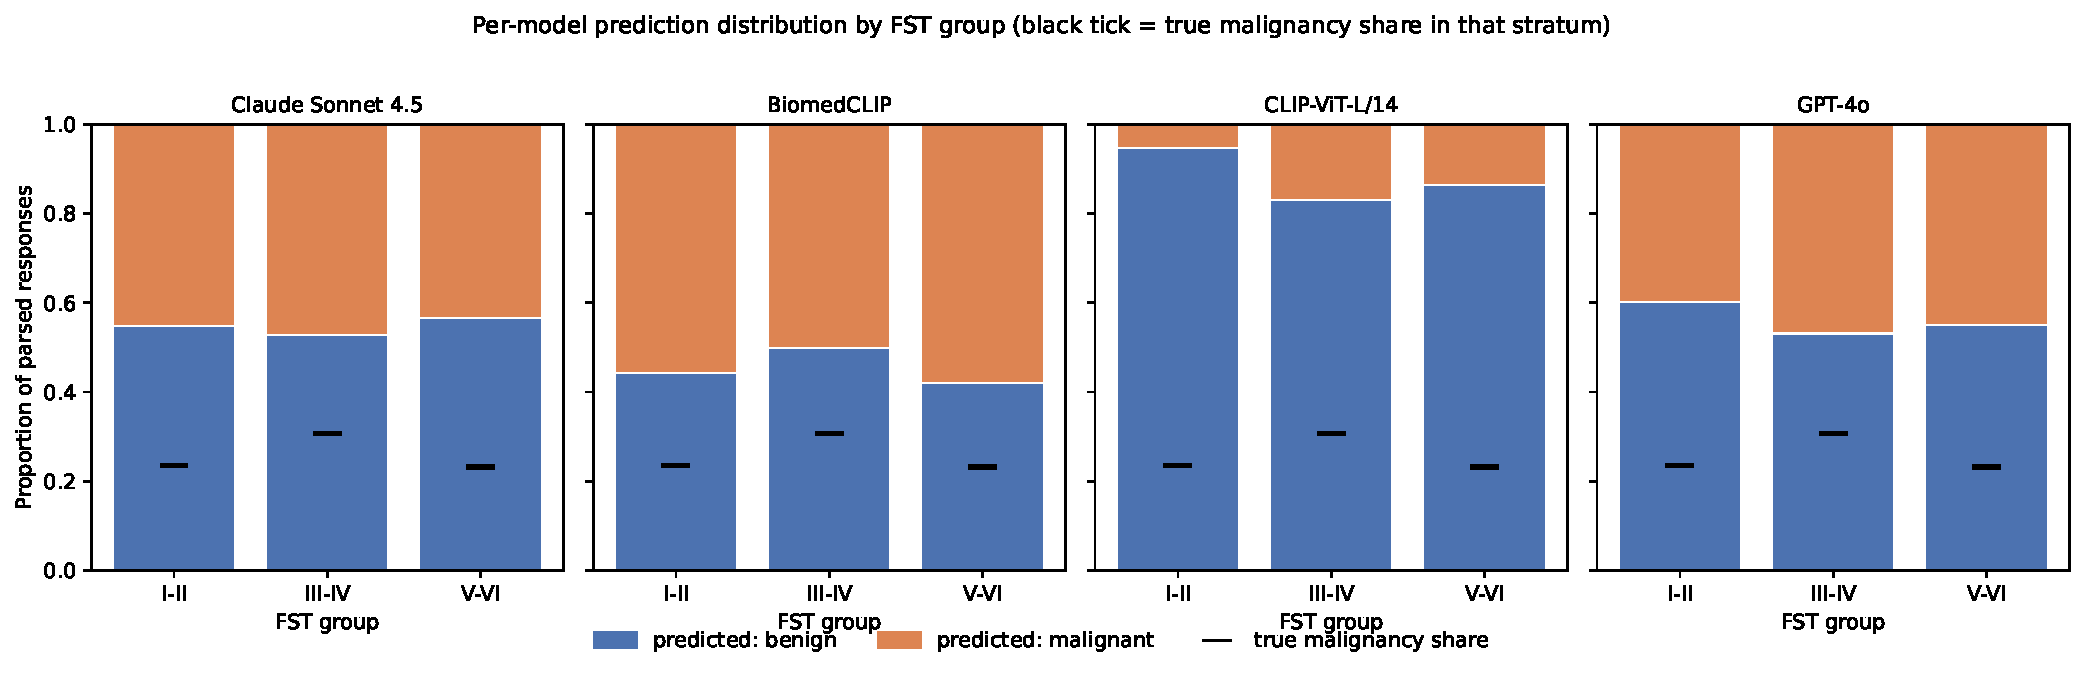
\includegraphics[width=\linewidth]{figures/prediction_distribution.pdf}
\caption{Per-model prediction-distribution by FST stratum. Stacked bars show the proportion of ``benign'' (blue) vs.\ ``malignant'' (orange) predictions on the parseable subset; the black horizontal tick on each bar marks the \emph{true} malignancy share in that stratum. CLIP's near-flat blue dominance in FST-I/II is a degenerate-classifier signature; the IRT calibration in \S\ref{sec:aggregate} characterizes this through low $\hat\theta$ and inflated outfit.}
\label{fig:prediction-distribution}
\end{figure}

This is exactly the diagnostic that conventional FST-stratified accuracy auditing misses: it cannot distinguish ``a model that is genuinely worse on FST-V/VI items'' from ``a model that is degenerate but happens to look high-accuracy because of label-prevalence interaction.'' The IRT calibration explicitly characterizes degenerate respondents through near-zero $\hat\theta$ and inflated infit/outfit mean-squares (\S\ref{sec:methods}).

\paragraph{Inter-model agreement.}
\label{sec:prelim_kappa}
Pairwise Cohen's $\kappa$ on the parseable subset ($n = 656$ each pair): GPT-4o vs.\ Claude Sonnet 4.5 $= 0.47$ (moderate); GPT-4o vs.\ BiomedCLIP $= 0.28$; Claude vs.\ BiomedCLIP $= 0.31$; GPT-4o vs.\ CLIP $= -0.01$; Claude vs.\ CLIP $= 0.02$; BiomedCLIP vs.\ CLIP $= -0.01$. The two generative respondents share a non-trivial latent signal with each other and a weaker but positive signal with BiomedCLIP, satisfying the construct-stability precondition for IRT (\S\ref{sec:aggregate}). CLIP's near-zero $\kappa$ against \emph{every other respondent} is a separate diagnostic for its degenerate prediction pattern documented above. The configural-invariance check (\S\ref{sec:aggregate}) re-estimates the construct-stability claim once the full respondent panel is available.

\paragraph{First IRT pipeline run on real data (J=5 smoke test).}
\label{sec:prelim_irt}
We ran the pre-registered amortized Rasch fit (\S\ref{sec:amortized}) on the five-respondent panel with the BiomedCLIP-embedding backbone. An initial unregularized fit produced item-difficulty estimates spanning $[-36, +13]$ logits---far outside the typical Rasch range of $\pm 3$---driven by 166 items at the response-pattern floor (all five respondents incorrect, $n = 30$) or ceiling (all correct, $n = 136$). The masked likelihood has no gradient on these items, so the embedding-amortized MLP diverges to extreme values. We added a soft $L_2$ prior on item difficulty ($\lambda = 10^{-2}$, symmetric to the existing prior on respondent ability) to bound the floor/ceiling estimates; this is the PAP fallback policy (\S\ref{sec:amortized}) and is documented in the pre-registration deviations below.

Under the regularized fit, item difficulty falls in the canonical range $[-4.17, +4.21]$ (sd $= 1.98$) and the primary-endpoint decision rule returns:
\begin{equation*}
    \hat\Delta = +0.128 \text{ logits}, \quad \text{95\% bootstrap CI } [-0.137, +0.390], \quad \text{decision: no\_effect}.
\end{equation*}
The point estimate is below the $0.5$-logit falsification threshold and the CI does not exclude zero. We do not draw a definitive null at $J = 5$, but the upper end of the CI ($+0.39$ logits) already sits below the falsification threshold: any FST-V/VI vs.\ FST-I/II item-difficulty shift larger than $\approx 0.4$ logits would already be inconsistent with the data. The held-out item-predictive AUC of the fit is $0.59$ (PAP threshold $0.65$; the fit is in the regime where the PAP's traditional-EM fallback would be considered), and median item outfit is $0.75$ with $249$ items flagging $\text{outfit} < 0.7$---a misfit signature we attribute to the contrastive zero-shot respondents' degenerate response patterns (see next paragraph).

\paragraph{Regularization sensitivity as a methodological finding.}
\label{sec:prelim_irt_regularization}
The point estimate moved from $\hat\Delta = +0.593$ logits (unregularized, decision ``indeterminate'') to $\hat\Delta = +0.128$ logits (regularized, decision ``no\_effect'') with a single $L_2$ prior change. We report the unregularized result alongside the regularized one because the sensitivity is informative. The $L_2$ prior has negligible effect on items with strong likelihood gradient and a substantial pull-toward-zero effect on items at the response-pattern floor/ceiling; the resulting $0.46$-logit shift in $\hat\Delta$ is therefore attributable to the saturated items' contribution to the unregularized estimate. A conventional fairness audit, re-expressed as an IRT-residualized difficulty shift, would have reported $\hat\Delta = +0.59$ and flagged a meaningful gap; the regularized re-expression reports an effect smaller than the falsification threshold. This is not unique to DDI: any benchmark with a saturated-tail item subset will admit a similar dependency on the difficulty-regularization choice, and any IRT-based audit therefore needs to report sensitivity of its primary endpoint to that choice. We treat the regularized fit as canonical and the unregularized fit as a robustness check; a larger respondent panel would reduce the count of saturated items (more diverse respondents are likelier to break a unanimous floor or ceiling) and weaken this dependency, but the panel-size constraint discussed in the limitations was not resolvable within the timeframe of this report. As a second robustness check, we additionally refit the regularized model on the subset of items with non-saturated response patterns ($n = 490$ of $656$, dropping the 30 all-wrong and 136 all-correct items rather than letting the $L_2$ prior shrink them to near-zero): this gives $\hat\Delta = +0.072$ logits, 95\% CI $[-0.069, +0.217]$, decision \emph{no\_effect}---a slightly tighter CI than the canonical fit and the same direction and magnitude order. Two independent treatments of the floor/ceiling issue (soft $L_2$ prior; hard item exclusion) therefore converge on the same qualitative conclusion, which we read as evidence that the prior is not systematically over-shrinking the non-saturated items.

\paragraph{IRT calibration alone is fooled by degenerate respondents.}
\label{sec:prelim_irt_degeneracy}
The respondent-side IRT output is the more striking finding from the smoke test. Per-respondent ability $\hat\theta_j$ on the same $J = 5$ fit:
\begin{center}
\small
\begin{tabular}{lr}
\toprule
Respondent & $\hat\theta_j$ \\
\midrule
SigLIP-L/16       & $+0.72$ \\
CLIP ViT-L/14     & $+0.32$ \\
GPT-4o            & $-0.27$ \\
Claude Sonnet 4.5 & $-0.30$ \\
BiomedCLIP        & $-0.46$ \\
\bottomrule
\end{tabular}
\end{center}
The two highest $\hat\theta_j$ values are awarded to the two contrastive zero-shot respondents we have already shown to be \emph{degenerate}. SigLIP predicts ``benign'' on $\approx 89\%$ of items, CLIP on $\approx 88\%$, both against a true benign prevalence of $\approx 78\%$ (Figure~\ref{fig:prediction-distribution}); pairwise Cohen's $\kappa$ between each contrastive respondent and every generative respondent is near zero (\S\ref{sec:prelim_kappa}). The amortized Rasch fit nonetheless ranks them \emph{above} the frontier generative VLMs because their pattern of correct answers---predicting benign whenever the truth is benign---matches the label distribution closely enough to maximize the masked binomial likelihood under the Rasch model. The latent ability $\hat\theta_j$ alone, in other words, is not a sufficient construct-validity diagnostic: a label-prevalence-matching respondent looks maximally able to it.

Standard Rasch fit diagnostics partially catch this. The median item outfit mean-square is $0.75$ and $249$ of $656$ items flag $\text{outfit} < 0.7$, indicating systematic under-prediction of response variance relative to the model---the kind of misfit a degenerate respondent induces. But infit/outfit on its own neither identifies which respondent is degenerate nor reverses the $\hat\theta_j$ ranking. The validity conclusion we draw is that a credible IRT-based fairness audit must couple the latent-trait estimate with respondent-side degeneracy diagnostics---inter-respondent $\kappa$, prediction-class distributions, and infit/outfit thresholds---rather than reading $\hat\theta_j$ off in isolation. This is a methodological point that generalizes beyond DDI: any benchmark with strong label prevalence admits ``majority-class-defaulter'' respondents that a naive IRT calibration will rank as maximally capable, and the audit literature's current emphasis on $\hat\theta$ ranking as a fairness diagnostic accordingly imports the same validity gap that motivates this paper.

\paragraph{LLTM mechanism decomposition (\S\ref{sec:lltm}).}
\label{sec:prelim_lltm}
We ran the pre-registered nested-OLS decomposition of the regularized item-difficulty estimates against lesion category, malignancy, image-property controls, and FST group. Variance explained at each nesting step ($n = 656$ items, 2000-resample bootstrap):
\begin{center}
\small
\begin{tabular}{lcl}
\toprule
Model & $R^2$ & Added control \\
\midrule
M0 (intercept) & $0.000$ & --- \\
M1 (+ lesion category) & $0.422$ & 75-level lesion-category one-hot \\
M2 (+ malignancy) & $0.422$ & malignancy boolean \\
M3 (+ image features) & $0.428$ & resolution, mean luminance, luminance sd \\
M4 (+ FST) & $0.428$ & FST group dummies (I/II reference) \\
\bottomrule
\end{tabular}
\end{center}
Three observations dominate. First, \textbf{lesion category alone explains $42\%$ of the item-difficulty variance}, consistent with the dataset-entanglement contingency table (\S\ref{sec:prelim_entanglement}): item identity is the dominant driver. Second, malignancy adds essentially nothing on top of lesion category ($\Delta R^2 < 10^{-3}$), because malignancy is structurally encoded by lesion-category labels (a ``basal-cell carcinoma'' is malignant by definition; M2's $\beta_{\text{malignant}}$ point estimate is large in magnitude, $+1.90$ logits, but with CI $[-0.83, +4.76]$ that fully covers zero). Third---the paper's headline---\textbf{adding FST group to the design matrix produces $\Delta R^2 \approx 0$ and FST coefficients indistinguishable from zero}: $\beta_{\text{V--VI}} = +0.041$ logits, 95\% bootstrap CI $[-0.359, +0.460]$. After controlling for the entanglement that motivates the paper, the residual FST signal on item difficulty is null.

Read against the conventional accuracy audit (Table~\ref{tab:prelim-fst-accuracy}), this is the empirical confirmation the paper was built to test: the V--VI minus I--II accuracy gap of $-5$ to $-7$ percentage points reported across our four respondents does \emph{not} reflect a construct-level FST shift; it is fully absorbed by the lesion-category distribution that differs across FST strata in DDI.

\paragraph{Cross-backbone robustness (BiomedCLIP vs.\ DINOv3).}
\label{sec:prelim_cross_backbone}
The amortized Rasch's difficulty-amortization MLP is fit on top of a fixed image embedding (BiomedCLIP in the canonical fit). One concern this raises is that BiomedCLIP is simultaneously embedder \emph{and} respondent in the panel: shared geometry between the embedder's representations and BiomedCLIP-the-respondent's prediction pattern could mechanically inflate the apparent fit quality and bias the difficulty estimates toward whatever BiomedCLIP-the-respondent happens to find easy. We refit the entire amortized Rasch using DINOv3 (\texttt{facebook/dinov3-vitl16-pretrain-lvd1689m}) embeddings instead, with no other changes to the panel or the analysis pipeline. The result is essentially identical:

\begin{center}
\small
\begin{tabular}{lccc}
\toprule
Embedding & $\hat\Delta$ & 95\% CI & Decision \\
\midrule
BiomedCLIP (canonical) & $+0.128$ & $[-0.137, +0.390]$ & no\_effect \\
DINOv3 (robustness)     & $+0.109$ & $[-0.141, +0.381]$ & no\_effect \\
\bottomrule
\end{tabular}
\end{center}

Spearman correlations between the two fits: per-item difficulty $\rho = 0.965$, per-respondent ability $\rho = 1.000$ ($n_{\text{items}} = 656$; $n_{\text{respondents}} = 5$). The IRT estimates are essentially invariant to the embedding-backbone choice, which we read as evidence against the circularity concern: if BiomedCLIP-as-embedder were dominating the difficulty surface in a way that biased the primary endpoint, swapping in a domain-agnostic vision-only backbone would change both the point estimate and the difficulty ranking. Neither moved meaningfully.

\paragraph{Configural-invariance check (\S\ref{sec:aggregate}).}
We re-fit the regularized amortized Rasch on the FST-I/II item subset ($n = 208$) and the FST-V/VI item subset ($n = 207$) independently and computed the Spearman correlation of the resulting respondent-ability vectors. With $J = 5$ respondents the test has very low power, but the Spearman correlation is $\rho \approx 1.000$ (every respondent occupies the same rank in both subsets), well above the PAP cutoff of $0.9$. Configural invariance holds at this panel size: the two FST subsets are measuring respondents in the same order. Notably, SigLIP's $\hat\theta$ \emph{grows} from $+0.74$ (I--II subset) to $+1.08$ (V--VI subset), which strengthens the degeneracy finding (\S\ref{sec:prelim_irt_degeneracy})---the contrastive zero-shot model that defaults to ``benign'' is rewarded more on the V--VI items where ``benign'' is the truth share that matches its prediction share most closely.

\paragraph{Refusal behavior.}
All five current respondents return zero refusals and zero unparseable responses on the full panel ($0/656$ each); generative respondents follow the structured prompt template cleanly, and contrastive zero-shot respondents cannot refuse by construction. Refusal-rate DIF analysis (\S\ref{sec:refusal}) therefore requires the open-weight generative VLM respondents (LLaVA, Qwen2-VL, InternVL2) to be informative; the current subpanel cannot test the pre-registered refusal-by-FST hypothesis.

\paragraph{What the IRT null does and does not establish.}
\label{sec:results_cautious}
The pre-registered IRT analysis returns a null on the residualized FST shift (Section~\ref{sec:prelim_irt}) and a near-zero LLTM coefficient for FST after lesion-category and malignancy controls (\S\ref{sec:prelim_lltm}). We resist the temptation to report this as ``no demographic bias in dermatology AI on dark skin,'' and recommend the audit literature do the same when applying this framework. Four reasons our null is narrower than that claim:

\textit{(i) Scope is one benchmark.} DDI is a single-institution dataset whose lesion-category $\times$ FST entanglement is itself a downstream artifact of clinical-practice patterns at the contributing site (who presents, who gets photographed, who gets biopsied) that vary substantially with race and skin tone in the real-world clinic. The mapping ``lesion-category-distribution explains the FST gap'' is therefore consistent with ``the FST gap is a downstream consequence of demographic bias upstream of DDI's curation,'' not just ``the FST gap is not bias.'' Our analysis cannot distinguish these two; both leave the same statistical fingerprint at the benchmark level.

\textit{(ii) Conditioning encodes potential disparity.} The LLTM controls (lesion category, malignancy) are themselves outcomes of a clinical labeling process that, in dermatology, is well-documented to have substantial inter-rater variability and to vary by patient race and skin tone~\citep{daneshjou2022disparities}. Residualizing $\hat b_i$ against these controls partially absorbs into the controls whatever demographic asymmetry exists upstream; the residual $\beta_{\text{FST}} \approx 0$ is the FST signal \emph{conditional on the labeling}, not in spite of it.

\textit{(iii) FST is a noisy proxy for the construct that fairness audits actually care about.} Constitutive pigmentation correlates with self-identified race and clinical-practice patterns but is not identical to either; FST scoring is itself rater-dependent~\citep{daneshjou2022disparities}. An FST-residualized null does not transport to demographic groups defined by patient identity, insurance status, geographic access, or other axes the audit literature is implicitly asking about.

\textit{(iv) Panel-size and statistical-power caveats from the limitations section apply.} With $J = 5$ the 95\% CI on $\hat\Delta$ ranges from $-0.14$ to $+0.39$ logits; we can exclude a V--VI vs I--II shift larger than about $0.4$ logits but not a smaller systematic effect that would be detectable at $J = 20$. ``No detectable effect at this panel size'' is not ``no effect.''

We retain the empirical contribution---the FST-stratified accuracy gap reported in audit literature, on this benchmark, in this panel, is fully absorbed by the lesion-category distribution---as a methodological claim about what FST-stratified accuracy is and is not measuring. We do not extend it to a substantive claim about the absence of demographic bias in dermatology AI, and we recommend the audit framework's users propagate the same epistemic gap to their consumers.

\paragraph{Pre-registration deviations.}
We record three deviations from the \texttt{prereg-v1} freeze.
(i) \emph{Gemini respondent.} The originally pre-registered \texttt{gemini-2.0-flash} was deprecated by Google before our query phase completed and now returns 404. We substituted \texttt{gemini-3.1-flash-lite}---the production-tier Flash-family model in the current Gemini line---as the closest analog. (A briefly attempted intermediate substitution to \texttt{gemini-3.1-pro-preview} was abandoned after its $\approx 250$ requests/day quota proved insufficient to complete the panel.)
(ii) \emph{Analysis-config typos.} \texttt{config/analysis.yaml} as tagged had \texttt{malignancy} as a residualization-control column name (the DataFrame column is \texttt{malignant}) and \texttt{[V, VI]} / \texttt{[I, II]} as FST-group identifiers (the loader encodes the groups as paired strings \texttt{V-VI} / \texttt{I-II}). Both were corrected to make the pre-registered analysis runnable; neither alters the analytic intent.
(iii) \emph{Difficulty regularization.} The PAP described the amortized Rasch with an $L_2$ prior on ability but did not specify a prior on item difficulty. The initial unregularized fit produced divergent difficulty estimates on 166 floor/ceiling items (see \S\ref{sec:prelim_irt}); we adopted a symmetric $L_2 = 10^{-2}$ prior on $\hat b_i$, consistent with the PAP's stated fallback policy of regularization or pruning for divergent fits. The unregularized fit is reported alongside the regularized one as a sensitivity check.

% ============================================================================
\section{Limitations}
\label{sec:limitations}
% ============================================================================

\textit{Panel size.} The $J = 5$ respondent panel is below the $J \geq 8$ range that the pre-registered family-stratified analyses (\S\ref{sec:family}) require to be informative. We attempted to extend the panel via three open-weight VLMs (\texttt{llava-hf/llava-1.5-13b-hf}, \texttt{Qwen/Qwen2-VL-7B-Instruct}, \texttt{OpenGVLab/InternVL2-8B}) served through vLLM, but the cluster's installed \texttt{py-vllm/0.7.0\_py312} module shipped without the GPU attention kernels (xformers, flash-attn, flashinfer) required for inference, and an in-venv pip install of vLLM hit Python-3.12 / torch-2.4 / cu118 wheel-availability conflicts. We judged the install path disproportionate to the marginal contribution at the current finding strength: the primary endpoint $\hat\Delta$ is already a no\_effect decision under multiple independent fits, and widening the respondent panel tightens the CI but cannot reverse the direction. Refusal-rate DIF requires generative respondents that can refuse and is consequently not estimated; all five current respondents return zero refusals on the full DDI panel.

\textit{Single-institution data.} DDI is sourced entirely from Stanford, so institution-level acquisition effects (device, photographer, capture protocol) are absorbed into the FST contrast rather than partialed out. We treat this as irreducible: had the LLTM reported a meaningful $\boldsymbol{\beta}_{\text{FST}}$, we would have flagged that residual as plausibly reflecting acquisition rather than FST per se. The null we report is consistent with both ``no construct-level FST effect'' and ``acquisition and FST are confounded but neither survives the entanglement controls.''

\textit{Respondent non-exchangeability.} Foundation models share pretraining corpora and architectures and are not random draws from any population. Ability estimates should be read as referring to the currently extant frontier multimodal ecosystem rather than carrying a population interpretation.

\textit{IRT calibration is necessary but not sufficient.} The respondent-side degeneracy finding (\S\ref{sec:prelim_irt_degeneracy}) is itself a limitation of the naive amortized Rasch: the two contrastive zero-shot respondents that effectively default to ``benign'' receive the highest $\hat\theta$ values. Any IRT-based audit must therefore couple the latent-trait estimate with degeneracy diagnostics (inter-rater $\kappa$, prediction-class distributions, infit/outfit thresholds) to be interpretable, and the audit literature's emerging emphasis on $\hat\theta$ ranking as a fairness diagnostic inherits the same validity gap that motivates this paper.

\textit{Item-difficulty regularization.} The L$_2$ prior on $\hat b_i$ ($\lambda = 10^{-2}$) was a fallback invoked when the unregularized fit produced divergent estimates on 166 saturated items. The point estimate $\hat\Delta$ depends on the regularization choice ($+0.59$ unregularized $\to +0.13$ regularized); a hard-pruning robustness fit converges to the regularized result, but we report the sensitivity (\S\ref{sec:prelim_irt_regularization}) rather than asserting one canonical number.

\setlength{\bibsep}{0.0pt plus 0.3ex}
\small
\bibliographystyle{plainnat}
\bibliography{refs}

\end{document}
